\documentclass{article}
\usepackage[english]{babel}
\usepackage{longtable}
\usepackage[top=1in, bottom=0.25in, left=1.25in, right=1.25in,includefoot,heightrounded]{geometry}
\usepackage{indentfirst}
\usepackage[utf8]{inputenc}
\usepackage{amsmath,amssymb}
\usepackage{graphicx,tikz}
\usepackage{hyperref}
\usepackage[colorinlistoftodos]{todonotes}
\usepackage[document]{ragged2e}
\usepackage{fancyhdr}
\usepackage{enumerate}
\usepackage{listings}
\usepackage{color}
\usepackage{flowchart}
\usepackage{graphicx}
\usetikzlibrary{arrows}

\usetikzlibrary{shapes.geometric, arrows}
\tikzstyle{startstop} = [rectangle, rounded corners, minimum width=3cm, minimum height=1cm,text centered, draw=black, fill=red!30]
\tikzstyle{decision} = [diamond, minimum width=4cm, minimum height=0.5cm, text centered, draw=black, fill=green!30]
\tikzstyle{process} = [rectangle, minimum width=3cm, minimum height=1cm, text centered, draw=black, fill=orange!30]
\tikzstyle{arrow} = [thick,->,>=stealth]
\tikzstyle{io} = [trapezium, trapezium left angle=70, trapezium right angle=110, minimum width=2cm, text width=4cm, minimum height=1cm, text centered, draw=black, fill=blue!30]

\pagestyle{fancy}
\fancyhf{}
\lhead{Myles Deslippe}
\rhead{CompTIA A+}
\cfoot{\thepage}

\definecolor{MyDarkGreen}{rgb}{0.0,0.4,0.0}
\lstset{inputencoding=ansinew}
\lstset{breaklines=true} 

\begin{document}

    \section*{\centering{Computers}}
    
    \subsection*{What is a Computer?}
    \begin{itemize}
        \item A \textbf{computer} is a \textbf{physical device designed to perform computation}.
        \item Laptops, mobile devices, and IoT devices are all computers.
    \end{itemize}
    
    \subsection*{What is an Operating System?}
    \begin{itemize}
        \item An \textbf{operating system} is a piece of \textbf{software} that \textbf{supports a computer's basic functions}. It manages tasks, applications, and controls peripherals.
        \item The \textbf{kernel} is the \textbf{heart of an operating system} that is responsible for \textbf{managing and providing services to processes}.
        \begin{itemize}
            \item One of the main responsibilities of the \textbf{kernel} is to manage the system's memory.
            \item Another responsibility is using drivers to communicate with controllers.
        \end{itemize}
    \end{itemize}

    \subsection*{Primary Computer Components}
    \begin{itemize}
        \item The \textbf{system unit} refers to the \textbf{physical computer} as a whole.
        \item The \textbf{monitor} is a \textbf{video output interface}.
        \item The \textbf{keyboard and mouse} are \textbf{input interfaces}.
        \item \textbf{Printers} provide a \textbf{paper output}.
        \item \textbf{Speakers} provide an \textbf{audio output}.
        \item \textbf{Microphones} provide an \textbf{audio input}.
        \item \textbf{Web cameras} provide a \textbf{visual input}.
    \end{itemize}

    \subsection*{External Connections}
    \begin{itemize}
        \item \textbf{Universal Serial Bus (USB)} is an \textbf{industry standard} that \textbf{establishes specifications for cables, connectors, and protocols for connection}.
        \begin{itemize}
            \item There are \textbf{different types} of \textbf{USB connections}.
        \end{itemize}
        \item \textbf{Ethernet} is a \textbf{technology for connecting devices} in a \textbf{wired local area network} or \textbf{wide area network}. \textbf{Ethernet connections} enable \textbf{different systems to communicate}.
        \begin{itemize}
            \item There are different types of ethernet connectors, the most common is \textbf{RJ45}.
        \end{itemize}
        \item \textbf{Audio jacks} are used to connect \textbf{input and output audio devices} to the \textbf{system unit}.
        \item There are \textbf{many kinds of video connections}, popular ones include:
        \begin{enumerate}
            \item \textbf{Digital Visual Interface (DVI)} is an older type of video connection.
            \item \textbf{High-Definition Multimedia Interface (HDMI)} is a type of video connection.
            \item \textbf{DisplayPort} is a modern type of video connector (typically used for high performance video output).
        \end{enumerate}
        \item \textbf{Mini-DIN (PS/2)} are older connections that allow \textbf{keyboards and mouses} to connect to older systems.
        \item \textbf{Parallel Port (LPT Port)} connectors are one of the oldest types of connectors, they are used to connect system units to \textbf{printers}.
        \item \textbf{Serial Connectors} are used for \textbf{inter-processor communication}, and are one of the oldest types of connections.
        \item \textbf{Video Graphics Array (VGA)} is an older type of video connector.
        \item \textbf{Separate Video (S-Video) Connectors} are an analog connector for standard definition video.
        \item[] \begin{center}
                    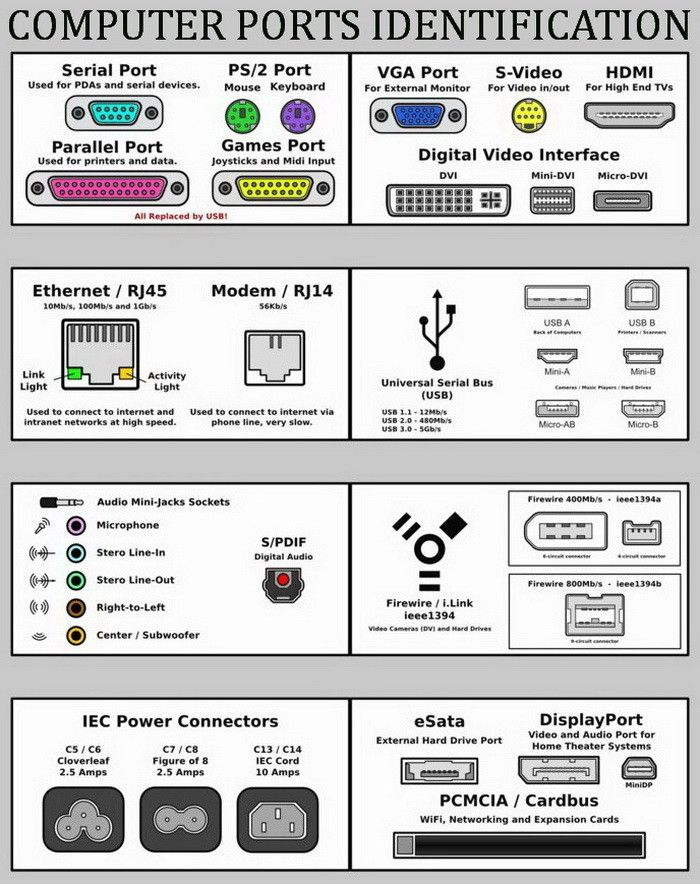
\includegraphics[width=(\textwidth / 2) - 15pt]{images/Connectors-1.jpg}
                    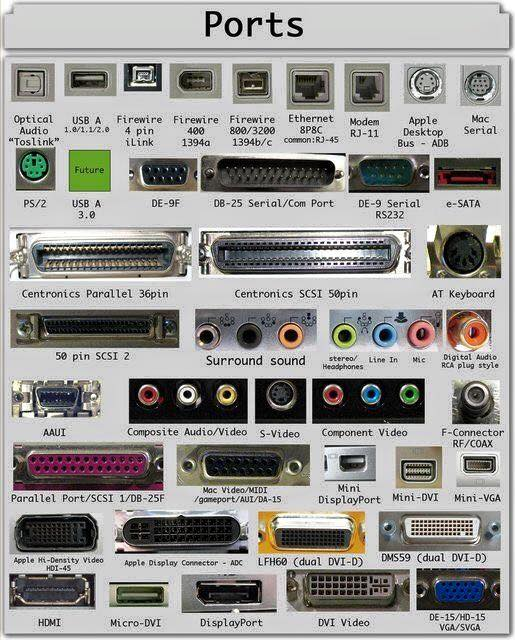
\includegraphics[width=(\textwidth / 2) - 15pt]{images/Connectors-2.jpg}
                \end{center}
    \end{itemize}


\end{document}